% %%%%%%%%%%%%%%%%%%%%%%%%%%%%%%%%%%%%%%%%%%%%%%%%%%%%%%%%%
% | - Electrochemical OER Application
% %%%%%%%%%%%%%%%%%%%%%%%%%%%%%%%%%%%%%%%%%%%%%%%%%%%%%%%%%
%
% __|
% %%%%%%%%%%%%%%%%%%%%%%%%%%%%%%%%%%%%%%%%%%%%%%%%%%%%%%%%%



% %%%%%%%%%%%%%%%%%%%%%%%%%%%%%%%%%%%%%%%%%%%%%%%%%%%%%%%%%
% | - Short Intro EChem Section
%
% __|
% %%%%%%%%%%%%%%%%%%%%%%%%%%%%%%%%%%%%%%%%%%%%%%%%%%%%%%%%%
% | - PARAGRAPH BODY
%
% TODO In the previous sections make sure to highlight the alpha and rutile IrO3 phases explicitly so that this sentence makes sense here.
Next, we performed \latin{ab-initio} thermodynamic analysis to test the OER electrochemical operational stability and activity of the most stable \IrOx in aqueous solution.
%
In particular, we compare the stability and activity of \rIrOtwo to our newly discovered \aIrOthree, and to the \rIrOthree polymorph.
%
In addition, we have also computed the stability and activity of a delithiated form of a recently reported $\beta$-Li\textsubscript{x}IrO\textsubscript{3} structure, referred here to as \bIrOthree.~\cite{Pearce2017,Pearce2019}
%
The OER activity was computed assuming the most common single-site associative OER mechanism and utilizing the limiting potential analysis and computational hydrogen electrode, as described extensively in numerous previous works\cite{Man2011,Rossmeisl2007,Kitchin2004, Bajdich2013} (see also Supporting Information for details).
% __|
% %%%%%%%%%%%%%%%%%%%%%%%%%%%%%%%%%%%%%%%%%%%%%%%%%%%%%%%%%


% %%%%%%%%%%%%%%%%%%%%%%%%%%%%%%%%%%%%%%%%%%%%%%%%%%%%%%%%%
% | - Bulk Pourbaix Diagram
%
% Explain the Ir and IrO[4-] species
% QUESTION Use E or U for potential variable
% __|
% %%%%%%%%%%%%%%%%%%%%%%%%%%%%%%%%%%%%%%%%%%%%%%%%%%%%%%%%%
% | - PARAGRAPH BODY
%
The calculated bulk Pourbaix diagram of the Ir-H\textsubscript{2}O system is shown in Figure~\ref{fig:bulk_pourbaix}.
%
The diagram was constructed by considering the thermodynamic equilibrium between the following species: Ir, \rIrOtwo, \aIrOthree, \rIrOthree, \bIrOthree, and an aqueous dissolved \ce{IrO^{4-}} species.
%
Not considering any of the \IrOthree in the bulk Pourbaix plots results in a completely different thermodynamic picture of \IrOtwo stability (Figure~\ref{fig:bulk_pourbaix_wo_alpha}).
%
To obtain free energies, we have utilized a free energy correction to our calculated values to reproduce the known experimental $\Delta H_f$ and $\Delta G_f$ of \rIrOtwo.~\cite{Barin1995}
%
While Ir and \rIrOtwo are most stable at low bias, \aIrOthree becomes the thermodynamically dominant phase under the relevant conditions for the OER (potentials $>$ \num{1.23} \VRHE and in an acidic environment).
%
% I want to be careful about how I talk about the metastable structures in the bulk Pourbaix, they strictly speaking shouldn't be there at all
The stability regions for less stable \bIrOthree and \rIrOthree phases,
in the absence of \aIrOthree, are also included,
and are indicated by solid lines.
%
It can be seen that these phases have a reduced, but sufficiently large, stability window relative to \IrOtwo and the \ce{IrO^{4-}}.
%
In total, we have discovered twenty-one unique \IrOthree polymorphs with a non-zero bulk Pourbaix stability region.
%
% TODO Create energy table for main bulk systems in SI
% The similar formation energies (see Table \ref{table:oer_table}) for all three \IrOthree species suggest some or all of these \IrOthree phases may be present and are stable under OER conditions.
% __|
% %%%%%%%%%%%%%%%%%%%%%%%%%%%%%%%%%%%%%%%%%%%%%%%%%%%%%%%%%


% =========================================================
% FIGURE ==================================================
% =========================================================
% | - Figure | Bulk Pourbaix Diagram
\begin{figure*}[!htb]
\centering
\makebox[\textwidth][c]{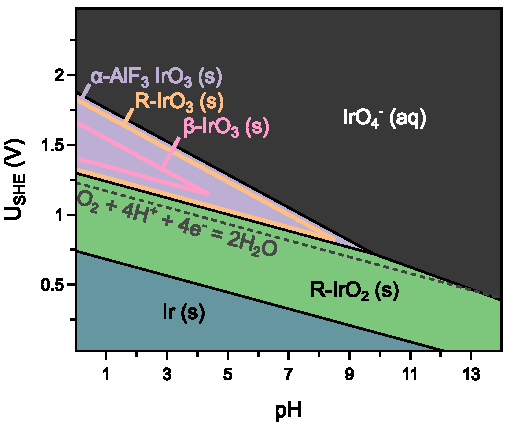
\includegraphics
{02_figures/oer_activity_stability/00_master__bulk-pourbaix__v6.pdf}}
\caption{\label{fig:bulk_pourbaix}
%
Revised bulk Pourbaix diagram of the \ce{Ir}-\ce{H2O} system as a function of applied potential and pH.
%
The diagram was constructed with Ir(s) (blue), \rIrOtwo (green), various \IrOthree polymorphs and a dissolved \ce{IrO^{4-}} ion species (dark grey).
%
The stability regions corresponding to the metastable \rIrOthree and \bIrOthree polymorphs (see text), in the absence of any competing \IrOthree phase, are displayed as yellow and pink lines, respectively.
%
The thermodynamic onset of OER (water equilibrium at \num{1.23} \VRHE) is also shown.
%
To be compared to Figure~\ref{fig:bulk_pourbaix_wo_alpha} without \IrOthree phases.
%
% The most stable system studied (see Table XX in SI for a full list) are Ir-metal Ir(s) (blue), a \rIrOtwo (green), and a dissolved \ce{IrO4[4-]} (grey).
%
% These are compared to the \ce{IrO_3} polymorphs, \aIrOthree (purple), \rIrOthree (orange), and \bIrOthree (pink).
}
\end{figure*}
% __| =====================================================
% =========================================================


% %%%%%%%%%%%%%%%%%%%%%%%%%%%%%%%%%%%%%%%%%%%%%%%%%%%%%%%%%
% | - Introduction to OER Results
%
% __|
% %%%%%%%%%%%%%%%%%%%%%%%%%%%%%%%%%%%%%%%%%%%%%%%%%%%%%%%%%
% | - PARAGRAPH BODY
%
The results of the electrochemical activity and surface stability analysis are summarized in Figure~\ref{fig:oer_volcano}.
%
There, in Figure~\ref{fig:oer_volcano}a, we report the surface energy Pourbaix plots and OER activity for various surface facets at selected coverages (for simplicity we only choose bare, 1ML OH* and 1ML O*) of all four systems from Figure \ref{fig:bulk_pourbaix}.
%
For each polymorph, surfaces were constructed by cleaving along the Miller indices with the highest calculated  diffraction peaks, corresponding to planes with higher density of atoms.
%
The surface stability Pourbaix plots identify which surface facets and surface coverage species are thermodynamically preferred under OER conditions.
%
Our results show, that most of the facets prefer to have a high surface coverage of O*, therefore we consider mainly oxygen terminated surfaces for the OER analysis.
%
Our results are comparable to previous studies on the electrochemical stability of \IrOtwo surfaces~\cite{Nattino2019,Raman2020},
but without considering highly reconstructed facets such as (101).
%
The surface stability analysis is therefore crucial for accurate determination of the activity.
% __|
% %%%%%%%%%%%%%%%%%%%%%%%%%%%%%%%%%%%%%%%%%%%%%%%%%%%%%%%%%


% =========================================================
% FIGURE ==================================================
% =========================================================
% | - Figure | OER Volcano/Surface Pourbaix
\begin{figure*}
\centering
\makebox[\textwidth][c]{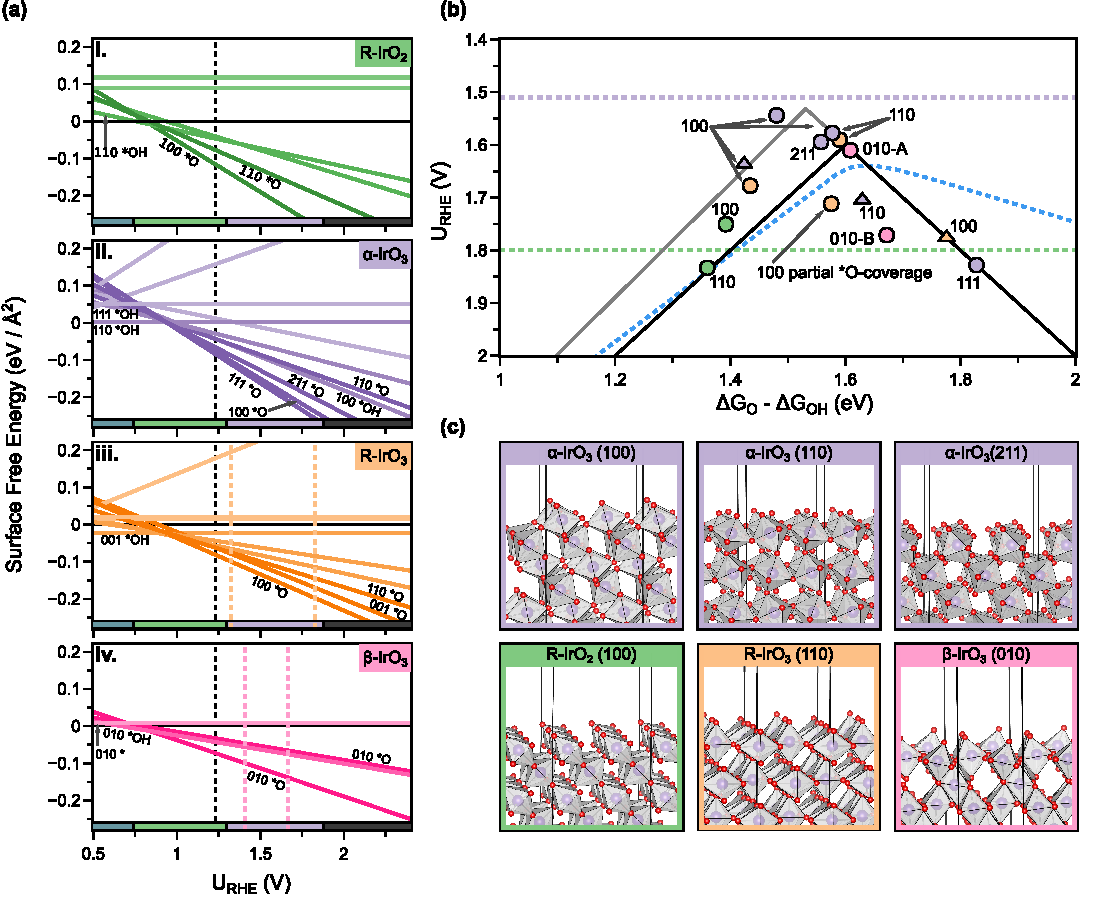
\includegraphics
{02_figures/oer_activity_stability/00_oer_plot_v10__downsampled_0900x0900.pdf}}
\caption{\label{fig:oer_volcano}
% TODO Insert green band into figure, insert experimental references for this
%
Summary of OER results for the following four bulk structures of \IrOx: \rIrOtwo (green), \aIrOthree (purple), \rIrOthree (orange), and \bIrOthree (pink).
%
(a) Surface energy Pourbaix diagrams for each structure, with the surface energy of various facets and coverages shown as a function of applied potential (\VRHE).
%
The coverage with bare surfaces (light lines), *OH covered  (medium lines) and *O covered surfaces (thick lines) are shown.
%
The bulk Pourbaix diagram's bounds of stability at pH \num{0} are superimposed as horizontal bars at the bottom of each subplot.
%
The pseudo-stability regimes for the meta-stable \bIrOthree and \rIrOthree are indicated by dashed vertical lines.
%
(b) OER activity volcano for \IrOx systems considered utilizing the \DGOmOH descriptor.
%
% TODO Add citations here
The horizontal lines correspond to recent experimental OER limiting potentials for \IrOtwo and \IrOthree~\cite{Seitz2016}, and were taken at a current density of \SI[mode=text]{10}{\mA\per\cm\squared}.
% The purple dotted line corresponds to the experimental limiting potential at \num{10} mA cm\textsuperscript{-2} for \ce{IrO_3} \cite{Seitz2016},
% while the green band corresponds to the range of experimentally observed overpotentials for pristine \ce{IrO_2} catalysts as reported in literature.
%
(c) Corresponding structural models for selected OER surfaces at 1ML O* coverage used for calculation of the overpotentials.
%
% (c) Select surface facets for the four \IrOx crystal systems considered.
%
Color legend: oxygen (red), purple (iridium), coordination motif (white).
}
\end{figure*}
% __| =====================================================
% =========================================================


% %%%%%%%%%%%%%%%%%%%%%%%%%%%%%%%%%%%%%%%%%%%%%%%%%%%%%%%%%
% | - OER Volcano
% TODO We don't mention new old/new scaling volcanos
% __|
% %%%%%%%%%%%%%%%%%%%%%%%%%%%%%%%%%%%%%%%%%%%%%%%%%%%%%%%%%
% | - PARAGRAPH BODY
%
% Replace G_O and G_OH with my custom macros for consistency
The calculated OER activities of relevant OER stable surfaces are
plotted against the \DGOmOH OER descriptor are shown in Figure \ref{fig:oer_volcano}b.
%
We display thermodynamic limiting potential volcano based on both the universal~\cite{Man2011} and fitted scaling (Figure ~\ref{fig:scaling_relations}) between \DGOOH with \DGOH, shown as solid lines.
%
Additionally, we have also added a kinetic OER volcano from Dickens \latin{et al.}~\cite{Dickens2019} based on the detailed microkinetic model developed for rutile systems, shown as the dashed line.
%
The kinetic volcano is constructed at the potential required to reach \SI[mode=text]{10}{\mA\per\cm\squared}.
%
The thermodynamic and kinetic volcanos agree remarkably well in the strong binding portion (left hand side) of the plot and exhibit similar optimum value, \DGOmOH $\approx$ \num{1.55}-\num{1.65} eV.
%
The corresponding surface structures for selected systems featuring high oxygen coverage are visualized in Figure \ref{fig:oer_volcano}c.

% __|
% %%%%%%%%%%%%%%%%%%%%%%%%%%%%%%%%%%%%%%%%%%%%%%%%%%%%%%%%%


% %%%%%%%%%%%%%%%%%%%%%%%%%%%%%%%%%%%%%%%%%%%%%%%%%%%%%%%%%
% | - TEMP

% __|
% %%%%%%%%%%%%%%%%%%%%%%%%%%%%%%%%%%%%%%%%%%%%%%%%%%%%%%%%%
% | - PARAGRAPH BODY
%
In general, the \rIrOtwo surfaces bind the OER intermediates relatively strongly, with theoretical limiting potentials of \mytilde\num{1.8} \VRHE (overpotential of \num{0.57} \VRHE) having the *O to *OOH potential limiting step, in agreement with previous theoretical studies.~\cite{Briquet2017,Strickler2019,Raman2020}
%
Based on the experimental values shown as horizontal line, the predicted overpotentials of our \rIrOtwo systems are also within the range of experimentally observed overpotentials.~\cite{Seitz2016, Kuo2017}.
%
The surfaces of the three \IrOthree polymorphs have \DGOmOH values shifted to higher energies, indicative of overall weaker binding energetics (see also Figure~\ref{fig:scaling_relations}).
%
On average, the adsorption of OH* and O* is weakened by \num{0.7} and \num{1.2} eV relative to \IrOtwo (Table~\ref{table:oer_data}), respectively.
%
The highest performing systems include the \aIrOthree (100), (110), and (211), followed by \bIrOthree (101), and then \rIrOthree (110).
%
These surfaces have overpotentials of \mytilde\num{0.4} \VRHE,
which represents a \mytilde\num{0.2} \VRHE improvement over \rIrOtwo, mirroring the observed shift in experimental onset potentials (horizontal lines).~\cite{Seitz2016, Kuo2017}.
%
The primary driver for the improved OER activity is the higher oxidation state of \IrOthree compared to \IrOtwo, having only three $5d$-electrons for \ce{Ir^{6+}} as opposed to five $5d$-electrons in  \ce{Ir^{4+}}, respectively.
%
Oxygen saturated \IrOthree systems thus bind OER intermediates more weakly, which leads to positive shift in \DGOmOH.
%
\IrOtwo and \RhOtwo are generally overbinding for OER~\cite{Dickens2019} so there is consequent improvement in OER activity when compared to these oxides.
%
These results are consistent with Back \latin{et al.}, who recently computed elevated activity in highly oxidized \IrOthree catalysts.\cite{Back2019}
%
An added feature of \aIrOthree is comparably higher density of active sites due to completely corner-sharing geometry.
%
The exact improvement in the theoretical overpotential is slightly dependent on the DFT level of theory and the inclusion of spin polarization, and has been discussed recently.~\cite{Seitz2016,Strickler2019}
% __|
% %%%%%%%%%%%%%%%%%%%%%%%%%%%%%%%%%%%%%%%%%%%%%%%%%%%%%%%%%
